% !TeX root = LAWRGe2023Notes.tex

In this lecture, we will study $Z(S^1)$, the \defterm{category of line operators} of our 3d TQFT.
The name ``line operator'' comes from the fact that a line is the link of $S^1$ in $\R^3$: %(see Figure \ref{fig:link_of_s1}).

\begin{figure}[htp]
    \centering
    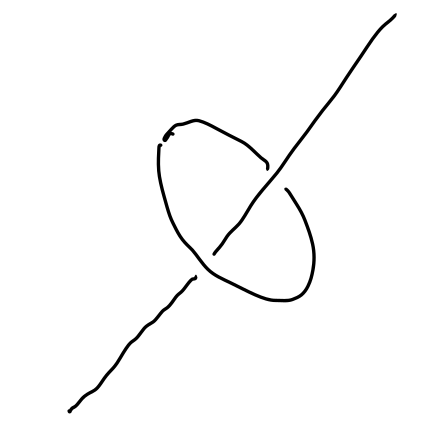
\includegraphics[width=2cm]{frilec1graphics/link.png}
\end{figure}

%\todo[inline]{Add figure!}

\subsection{General Structure of Line Operators}

Note that $Z(S^1)$ is a linear category, and objects $\ell \in Z(S^1)$ are used to ``firm up'' surfaces.
More precisely, if $\Sigma$ is a surface with holes, and to each hole we assign some $\ell_i \in Z(S^1)$, then we obtain a \emph{vector space} $Z(\Sigma; \ell_1, \dots, \ell_n)$.

Morphisms in $Z(S^1)$ are defined as follows.
Consider the cylinder $C = S^1 \times [0, 1]$ as having two incoming boundary components and no outgoing boundary.
If we place a line operator $\ell_i$ ($i = 1, 2$) at each boundary component,
we get %\todo{add figures!}
\begin{equation}
Z(C; \ell_1, \ell_2) = \Hom_{Z(S^1)}(\ell_1, \ell_2).
\end{equation}
This corresponds to the following cobordism:
\begin{figure}[htp]
    \centering
    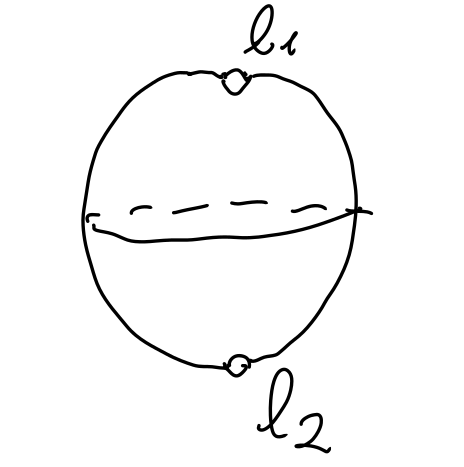
\includegraphics[width=3cm]{frilec1graphics/hom.png}
\end{figure}

\noindent We can view $Z(C)$ as the functor
\begin{equation}
Z(C) = \Hom_{Z(S^1)}(-, -).
\end{equation}

\noindent The product on $Z(S^2)$ comes from sticking small disks $D^3_1$, $D^3_2$ inside a larger disk $D^3$:
\begin{figure}[htp]
    \centering
    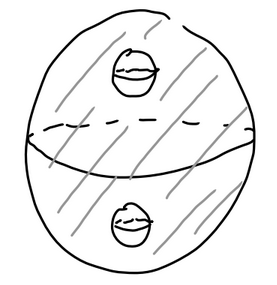
\includegraphics[width=3cm]{frilec1graphics/E3mult.png}
\end{figure}

\noindent This defines a cobordism $D^3 \setminus (\mathring{D}^3_1 \sqcup \mathring{D}^3_1): S^2_1 \sqcup S^2_2 \to S^2$
%\todo{add figure!}
which gives an $\E_3$ multiplication on $S^2$.

We can adapt this picture to get a description of composition of morphisms in $Z(S^1)$.
Namely, the surface (topologically a torus)
\begin{figure}[!htp]
    \centering
    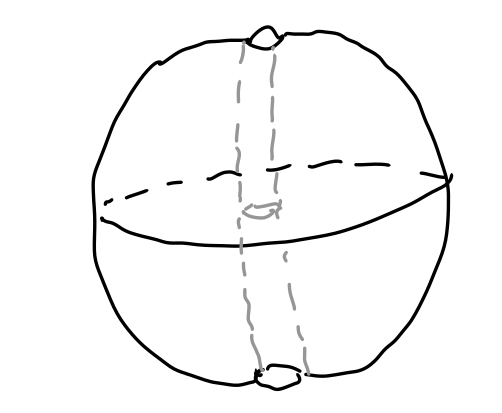
\includegraphics[width=3cm]{frilec1graphics/compos.png}
\end{figure}

\noindent defines the composition map
\begin{equation}
\circ: \Hom_{Z(S^1)}(\ell_2, \ell_3) \otimes \Hom_{Z(S^1)}(\ell_1, \ell_2) \to \Hom_{Z(S^1)}(\ell_1, \ell_3).
\end{equation}

The category $Z(S^1)$ has an $\E_2$-structure.
In other words, we can view $Z(S^1)$ as a braided tensor category.
This structure comes from the following morphisms:%\todo{add figures!}
\begin{itemize}
    \item A tensor operation $\otimes: Z(S^1) \boxtimes Z(S^1) \to Z(S^1)$ defined by
    \begin{figure}[htp]
    \centering
    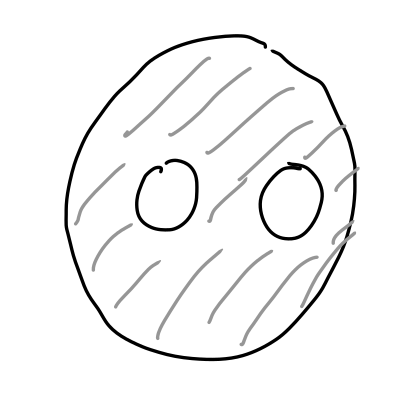
\includegraphics[width=3cm]{frilec1graphics/mult.png}
\end{figure}
    \item A braiding defined by
    \begin{figure}[htp]
    \centering
    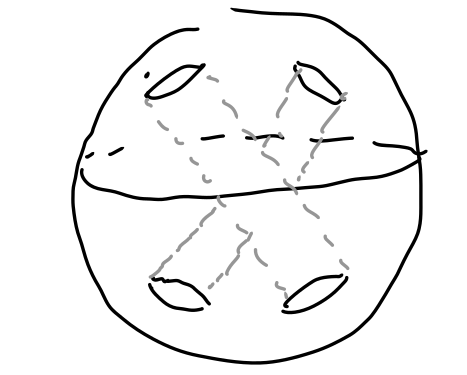
\includegraphics[width=3cm]{frilec1graphics/braiding.png}
\end{figure}
    \item A tensor unit $\mathbbm{1} \in Z(S^1)$, the \defterm{trivial} or \defterm{identity line}, defined by
    \begin{figure}[htp]
    \centering
    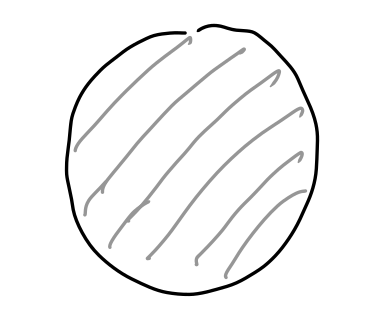
\includegraphics[width=3cm]{frilec1graphics/unit.png}
\end{figure}
\end{itemize}

The category $Z(S^1)$ has an $S^1$-action coming from the group $S^1$ acting on the manifold $S^1$ by rotation.
Passing to $S^1$-invariants (in physics language, ``turning on an Omega background'') takes us from an $\E_2$-category to an $\E_0$-category (i.e. a category with a distinguished object $\mathbbm{1}$).
One can compare this to how taking $S^1$-invariants sends the $\E_3$-algebra $Z(S^2)$ to an $\E_1$-algebra.

\subsection{State Spaces from $Z(S^1)$}

We can recover the value of $Z$ on a surface (or a $3$-manifold) from $Z(S^1)$.

\begin{example}
To compute $Z(S^2)$, we note
\begin{equation}
Z(S^2) = Z(D^2 \cup_{S^1} D^2) = \Hom_{Z(S^1)}(Z(D^2), Z(D^2)) = \Hom_{Z(S^1)}(\mathbbm{1}, \mathbbm{1}) = \mathrm{End}_{Z(S^1)}(\mathbbm{1}).
\end{equation}
From the physics of $3$d $\cN = 4$ gauge theories, we know that $Z(S^2) = \C[\cM_{\mathrm{vac}}]$.
If we know $\cM_{\mathrm{vac}}$ (or its affinization $\cM_{\mathrm{vac}}^{\mathrm{aff}}$), this gives us a good check for proposed definitions of $Z_A(S^1)$ and $Z_B(S^1)$.
\end{example}

Consider the functor\footnote{Here we are making explicit the previously implicit assumption that the categories appearing in the study of $3$d $\cN = 4$ gauge theories are all derived / dg-categories.}
\begin{equation}
\Hom_{Z(S^1)}(-, \mathbbm{1}): Z(S^1)^{\mathrm{op}} \to \C[\cM_{vac}]-\mod = \bfD^b\big(\mathrm{Coh}(\cM_{\mathrm{vac}}^{\mathrm{aff}})\big).
\end{equation}
If $\cM_{\mathrm{vac}}$ is smooth, renormalization group flow arguments tell us that this functor should be an equivalence.
In general, $Z(S^1)$ will contain more information than $\bfD^b\big(\mathrm{Coh}(\cM_{\mathrm{vac}}^{\mathrm{aff}})\big)$, e.g.\ $Z(S^1)$ controls deformations and resolutions of $\cM_{\mathrm{vac}}^{\mathrm{aff}}$.

\begin{example}
To compute $Z(T^2)$, we note
\begin{equation}
Z(T^2) = Z\big((S^1 \times [0, 1]) / ((x, 0) \sim (x, 1)\big) = \textrm{``trace of Hom''} := \mathrm{HH}_\bullet(Z(S^1)), 
\end{equation}
the Hochschild homology of the category $Z(S^1)$.
The ``trace'' here can be understood using the picture of beads on a string
\begin{figure}[htp]
    \centering
    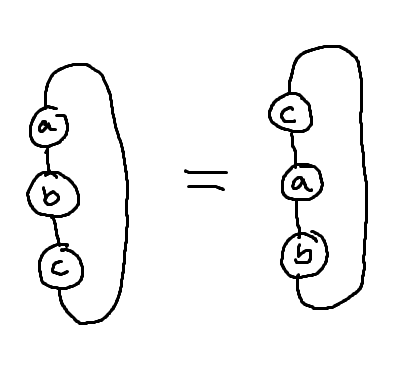
\includegraphics[width=3cm]{frilec1graphics/trace.png}
\end{figure}

\noindent where the ``beads'' (here $a, b, c$) are homomorphisms, and the picture defines the trace of the composite (here $\mathrm{tr}(abc) = \mathrm{tr}(cab)$).
\end{example}

\subsection{Line Operators in Topological Twists: Strategy}

To compute $Z(S^1)$ for the A- or B-twists of the $3$d $\cN = 4$ gauge theory corresponding to $G$ and $T^* V$ (where $\rho: G \to \mathrm{U}(V)$ is a unitary representation), we proceed by:
\begin{enumerate}
    \item Solving the equations of motion for the A- or B-twist.
    \item ``Quantizing,'' roughly by:
    \begin{enumerate}
        \item (A-twist) taking the Fukaya category of the moduli space of solutions.
        \item (B-twist) taking $\bfD^b \mathrm{Coh}$ of the moduli space of solutions.
    \end{enumerate}
\end{enumerate}
We will work this out in more detail as follows.

\subsection{Line Operators in the $3$d B-Model}

Fix coordinates $\vec{X}, \vec{Y}$ on $T^* V = V \oplus V^*$, and write a general $G_\C$-connection as $\cA$.
The equations of motion of the $B$-twist are given by setting $Q_B(-) = 0$ for all fields.
This yields:
\begin{equation}
    \begin{cases}
        \cF_\cA = 0 \\
        \mathrm{d}_\cA \vec{X} = \mathrm{d}_\cA \vec{Y} = 0 \\
        \mu_\C(\vec{X}, \vec{Y}) = \rho^*(\vec{X}, \vec{Y}) = 0 \\
        \textrm{a reality equation}
    \end{cases}
\end{equation}
To find the moduli space of solutions, we must quotient by $G$-gauge transformations.
In fact, it is more convenient to quotient by $G_\C$-gauge transformations, which removes the reality equation.

In an infinitesimal neighborhood of $S^1$ in $\R^3$, the only information in the connection $\cA$ is the holonomy $g = \mathrm{Hol}_{S^1_p}(\cA) \in G_\C$ for some point $p \in S^1$.
Let $\vec{X}_p$ and $\vec{Y}_p$ be the values of the fields $\vec{X}$ and $\vec{Y}$ at $p$.
Our equations of motion become
\begin{equation}
\begin{cases}
    g \vec{X}_p = \vec{X}_p \\
    \vec{Y}_p g^{-1} = \vec{Y}_p \\
    \mu_\C(\vec{X}_p, \vec{Y}_p) = 0.
\end{cases}
\end{equation}

It is a good exercise to check that these equations are equivalent to the single equation $\mathrm{d} W = 0$ for $W: G_\C \times V \times V^* \to \C$ given by
\begin{equation}
W(g, \vec{X}, \vec{Y}) = \vec{Y} \cdot (\rho(g) - 1) \vec{X}.
\end{equation}
Thus the moduli space of solutions is
\begin{equation}
\Big\{ \big(g, \vec{X}, \vec{Y}\big) \in G_\C \times V \times V^* \, \Big| \, \mathrm{d}_{(g, \vec{X}, \vec{Y})} W = 0 \Big\} / G_\C.
\end{equation}
Here $h \in G_\C$ acts by $h \cdot (g, \vec{X}, \vec{Y}) \mapsto (h g h^{-1}, h \vec{X}, \vec{Y} h^{-1})$.

The resulting moduli space is typically singular, so it is better to use the category of (equivatiant) matrix factorizations than the category of coherent sheaves.
Thus
\begin{equation}
Z^B_{G,V}(S^1) = \mathrm{MF}^{G_\C}\Big(\Big\{ \big(g, \vec{X}, \vec{Y}\big) \in G_\C \times V \times V^* \, \Big| \, \mathrm{d}_{(g, \vec{X}, \vec{Y})} W = 0 \Big\}\Big)
\end{equation}
Here $\mathbbm{1} = \cO_{g=1}$, and $\mathrm{End}(\mathbbm{1}) = \C[T^* V // G_\C] = \C[\cM_H]$.

\begin{example}
Consider the case where $G = 1$ and $V = \C$.
The moduli space of solutions is smooth in this case, so we can use coherent sheaves in place of matrix factorizations, and
\begin{equation}
Z^B_{1,\C}(S^1) = \bfD^b \mathrm{Coh}(T^* \C),
\end{equation}
Here $\mathbbm{1} = \O_{T^* \C}$ and $\mathrm{End}(\mathbbm{1}) = \C[T^* \C]$.

It is more interesting to note that
\begin{equation}
Z^B_{1,\C}(T^2) = \mathrm{HH}_\bullet(\bfD^b \mathrm{Coh}(T^* \C)) = \C[X, Y, \mathrm{d}\overline{X}, \mathrm{d}\overline{Y}]
\end{equation}
by the Hochschild-Kostant-Rosenberg theorem.
Here $X$ and $Y$ are in even degree, and $\mathrm{d}\overline{X}$ and $\mathrm{d}\overline{Y}$ are in odd degree.
\end{example}

\subsection{Line Operators in the $3$d A-Model}

If we think algebraically and ``squint hard enough,'' an infinitesimal neighborhood of $S^1$ in $\R^3$ looks like $D^\times = \mathrm{Spec} \C((z))$.
The moduli space solutions to the $3$d A-model equations of motion on $D^\times$ look like $T^*\big(V((z)) / G_\C((z)) \big)$, where the quotient by $G_\C((z))$ corresponds to modding out by gauge equivalence.

We expect $Z^A_{G,V}(S^1)$ to be something like the Fukaya category of this moduli space, but this is hard to define rigorously.
Work of Justin Hilburn and Philsang Yoo proposes that we instead consider the category of $D$-modules (or constructible sheaves) on the base of the cotangent bundle.
The modified proposal is then
\begin{equation}
Z^A_{G,V}(S^1) = D-\mod\big(V((z)) / G_\C((z))\big) = D-\mod^{G_\C((z))}\big(V((z))\big),
\end{equation}
the category of strongly equivariant $D$-modules on $V((z))$.

This definition may look abstract, but it is compatible with the BFN construction of Coulomb branches, providing evidence for its validity.
Basic objects of $Z^A_{G,V}(S^1)$ are labeled by pairs
\begin{equation}
\{ (L \subset V((z)) \textrm{ a subspace}, H \subset G_\C((z))\textrm{ a subgroup}) \, | \, H \textrm{ stabilizes } L \}.
\end{equation}
Here
\begin{align}
\Hom_{Z^A_{G,V}(S^1)}\big((L, H), (L', H')\big) &= \mathrm{H}_\bullet((L' / H') \times_{V((z)) / G_\C((z))} L / H) \\
&= \mathrm{H}_\bullet \left(H' \backslash \{ (\vec{X}, \vec{X}', g) \in L \times L' \times G_\C((z)) \, | \, \vec{X}' = g \vec{X} \} / H\right).
\end{align}
The unit object $\mathbbm{1}$ is given by the pair $(V[[z]], G_\C[[z]])$ (this is an algebraic version of ``filling in $D^\times$ to $D$'').
One can check that $\mathrm{End}(\mathbbm{1}) = \C[\cM_C]$, as claimed above.

\subsection{$3$d Mirror Symmetry for Line Operators}

Mirror symmetry results have been proven for categories of line operators in the case when $G$ is abelian.
We discuss some of them here.

\begin{Theorem}[Hilburn, Raskin]
There exists an equivalence of categories between $Z^A_{1,\C}(S^1)$ and a de Rham version of $Z^B_{U(1), \C}(S^1)$.
\end{Theorem}

This theorem can be extended to other examples by looking at the behavior of the tensoring operation and the action of hyperk\"ahler isometries.

Another approach proceeds by interpreting line operators in terms of vertex algebras.

\begin{Theorem}[Ballin, Creutzig, Dimofte, Niu]
If $G$ is abelian and $G \curvearrowright V$ is faithful, then
\[
Z^B_{G,V}(S^1)^{\mathrm{finitely \,\, supported \,\, on \,\,} G_\C} \simeq \bfD^b(\mathrm{modules \,\, over \,\, some \,\, VOA})
\]
as braided tensor categories.
Furthermore, there is a $3$d mirror symmetry statement relating this to an A-side category of VOA modules contained in $Z^A_{G^!,V^!}(S^1)$.
\end{Theorem}

The slogan of this theorem is that $3$d mirror symmetry for line operators looks like $2$d mirror symmetry on loop spaces.

The nonabelian case is poorly understood, and work on understanding it is highly desirable.
One viewpoint on the nonabelian case comes from Ben Webster's work interpreting $3$d mirror symmetry combinatorially using KLRW algebras.

\begin{Theorem}[Webster]
When $\cM_C$ admits a full resolution $\widetilde{\cM_C} \to \cM_C$, there exists a deformation of $Z^A_{G,V}(S^1)$ to $\bfD^b\big(\mathrm{Coh}(\widetilde{\cM_C})\big)$.
\end{Theorem}

This is a non-abelian mirror symmetry statement, but it misses information about the singularities.
The deformation here is mirror to the deformation of $Z^B_{G^!, V^!}(S^1)$ obtained by imposing GIT stability parameters.
It would be good to have an improved version of this theorem incorporating the full category of line operators in the $A$-model and singularities of the moduli space.

\subsection{Exercises}

\begin{exercise}
Suppose that $G=U(1)$ acts on $V=\C^2$ with weights $(1,3)$. (In other words $e^{i\theta}:(X^1,X^2)\mapsto (e^{i\theta}X^1,e^{3i\theta}X^2)$.)

Write down explicitly the superpotential
%
$$  W : G_\C \times V \times V^* \to \C $$
%
that appears in the solution to the B-twist equations of motion on $S^1$. Differentiate with respect to $g\in G_\C$ to recover the complex moment map $\mu_\C$ for the action on $T^*V$.

\end{exercise}

For the remaining problems, recall that in the A twist of $(G,T^*V)$ gauge theory, the category $Z(S^1)$ has (some) objects labelled by $(L,H)$ where $L$ is a subspace of $V(\!(z)\!)$, and $H$ is a subgroup of $G_\C(\!(z)\!)$ that stabilizes $L$. The morphism space between two such objects may be defined as Borel-Moore homology
%
$$ \text{Hom}\big((L,H),(L',H')\big) := H_\bullet\Big(  H'\big\backslash\big\{ (X',X,g)\in L'\times L\times G_\C(\!(z)\!)\,\big|\, X'=gX\big\}\big/H \Big) $$
%
Note that when a quotient is not free (as in the $H$ or $H'$ quotients above) it should be interpreted as taking equivariant cohomology.

\begin{exercise}

Let $1\!\!1 := (V[\![z]\!],G_\C[\![z]\!])$. Argue that $\text{End}(1\!\!1) = \C[\cM_C]$ reproduces the BFN construction of the Coulomb branch.

\end{exercise}

\begin{exercise}
Take $G=U(1)$ and $V=\C$ (with weight $1$). Recall that the Coulomb branch algebra may be presented as
%
$$ \C[\cM_\C] \simeq \C[v_+,v_-,\varphi]/(v_+v_-=\varphi)\,. $$
\end{exercise}
%
Consider line operators
%
$$ \cN_+ = (\C(\!(z)\!),\C(\!(z)\!)^*)\,,\qquad  \cN_- = (0,\C(\!(z)\!)^*)\,. $$
%
Show that they give rise to modules
%
$$ \text{Hom}(\cN_+,1\!\!1) = \C[\cM_C]/(v_+-1)\,,\qquad \text{Hom}(\cN_i,1\!\!1) = \C[\cM_C]/(v_--1)\,. $$

\end{document}